\documentclass[conference]{IEEEtran}
\IEEEoverridecommandlockouts

\usepackage{cite}
\usepackage{amsmath,amssymb,amsfonts}
\usepackage{algorithmic}
\usepackage{graphicx}
\usepackage{booktabs}
\usepackage{textcomp}
\usepackage{xcolor}
\usepackage{url}
\usepackage{hyperref}
\usepackage{tikz}
\usetikzlibrary{positioning,arrows.meta,calc,fit,backgrounds}

\graphicspath{{figs/}{../results/}{../results/eda/}}

\tikzset{
  block/.style={draw, rounded corners=2pt, align=center, font=\footnotesize,
    minimum height=7mm, inner sep=2pt},
  enc/.style    ={block, fill=gray!18, minimum width=24mm},
  fuse/.style   ={block, fill=blue!8,  minimum width=28mm},
  bit/.style    ={block, fill=orange!18, minimum width=28mm},
  head/.style   ={block, fill=green!12, minimum width=16mm,
    minimum height=6mm, font=\scriptsize},
  loss/.style   ={block, dashed, fill=gray!5, font=\scriptsize,
    minimum width=30mm, minimum height=6mm},
  io/.style     ={font=\footnotesize},
  arr/.style    ={-{Stealth[length=1.5mm,width=1.2mm]}, semithick},
  label/.style  ={font=\scriptsize\itshape, midway, fill=white,
    inner sep=1pt}
}

\begin{document}

\title{Multi-Label Bitemporal Change Classification\\
  with Long-Tail Object, Event, and Attribute Heads}

\author{
  \IEEEauthorblockN{Yasin TODO\_SURNAME}
  \IEEEauthorblockA{Y\i ld\i z Technical University\\
    BLM5135 -- Deep Learning and Neural Networks Fundamentals\\
    Spring 2026}
}

\maketitle

\begin{abstract}
% 4-5 sentences. Problem, method, key result.
We address multi-label change classification on bitemporal aerial RGB image
pairs with three independent label families: 12 object classes, 12 event
classes, and 24 attribute classes (totalling 48 sigmoid heads). The dataset
is severely long-tailed -- the most frequent object class has 270x more
positives than the rarest. We train two model families under the same
ConvNeXt-V2 Tiny Siamese backbone: (i) three single-task Phase~1 models
with a four-way fusion (concatenation, absolute difference, Hadamard) and
asymmetric loss, and (ii) a unified Phase~2 model adding a Bitemporal
Image Transformer (BIT) fusion and a fixed-weight multi-task head. Phase~1
reaches 0.277 mean macro-F1 over three seeds; Phase~2 reaches 0.282,
with BIT contributing both a small mean gain and a halving of cross-seed
variance. We report all ablations -- including ones that did not help
(no-change gate, Query2Label heads, uncertainty-weighted loss) -- as
negative results.
\end{abstract}

\begin{IEEEkeywords}
multi-label classification, change detection, long-tail learning, vision
transformer, bitemporal imagery.
\end{IEEEkeywords}

% =====================================================================
\section{Introduction}
% 0.5 page. Bitemporal change task, multi-label setup, long tail,
% contributions.

\begin{figure}[t]
  \centering
  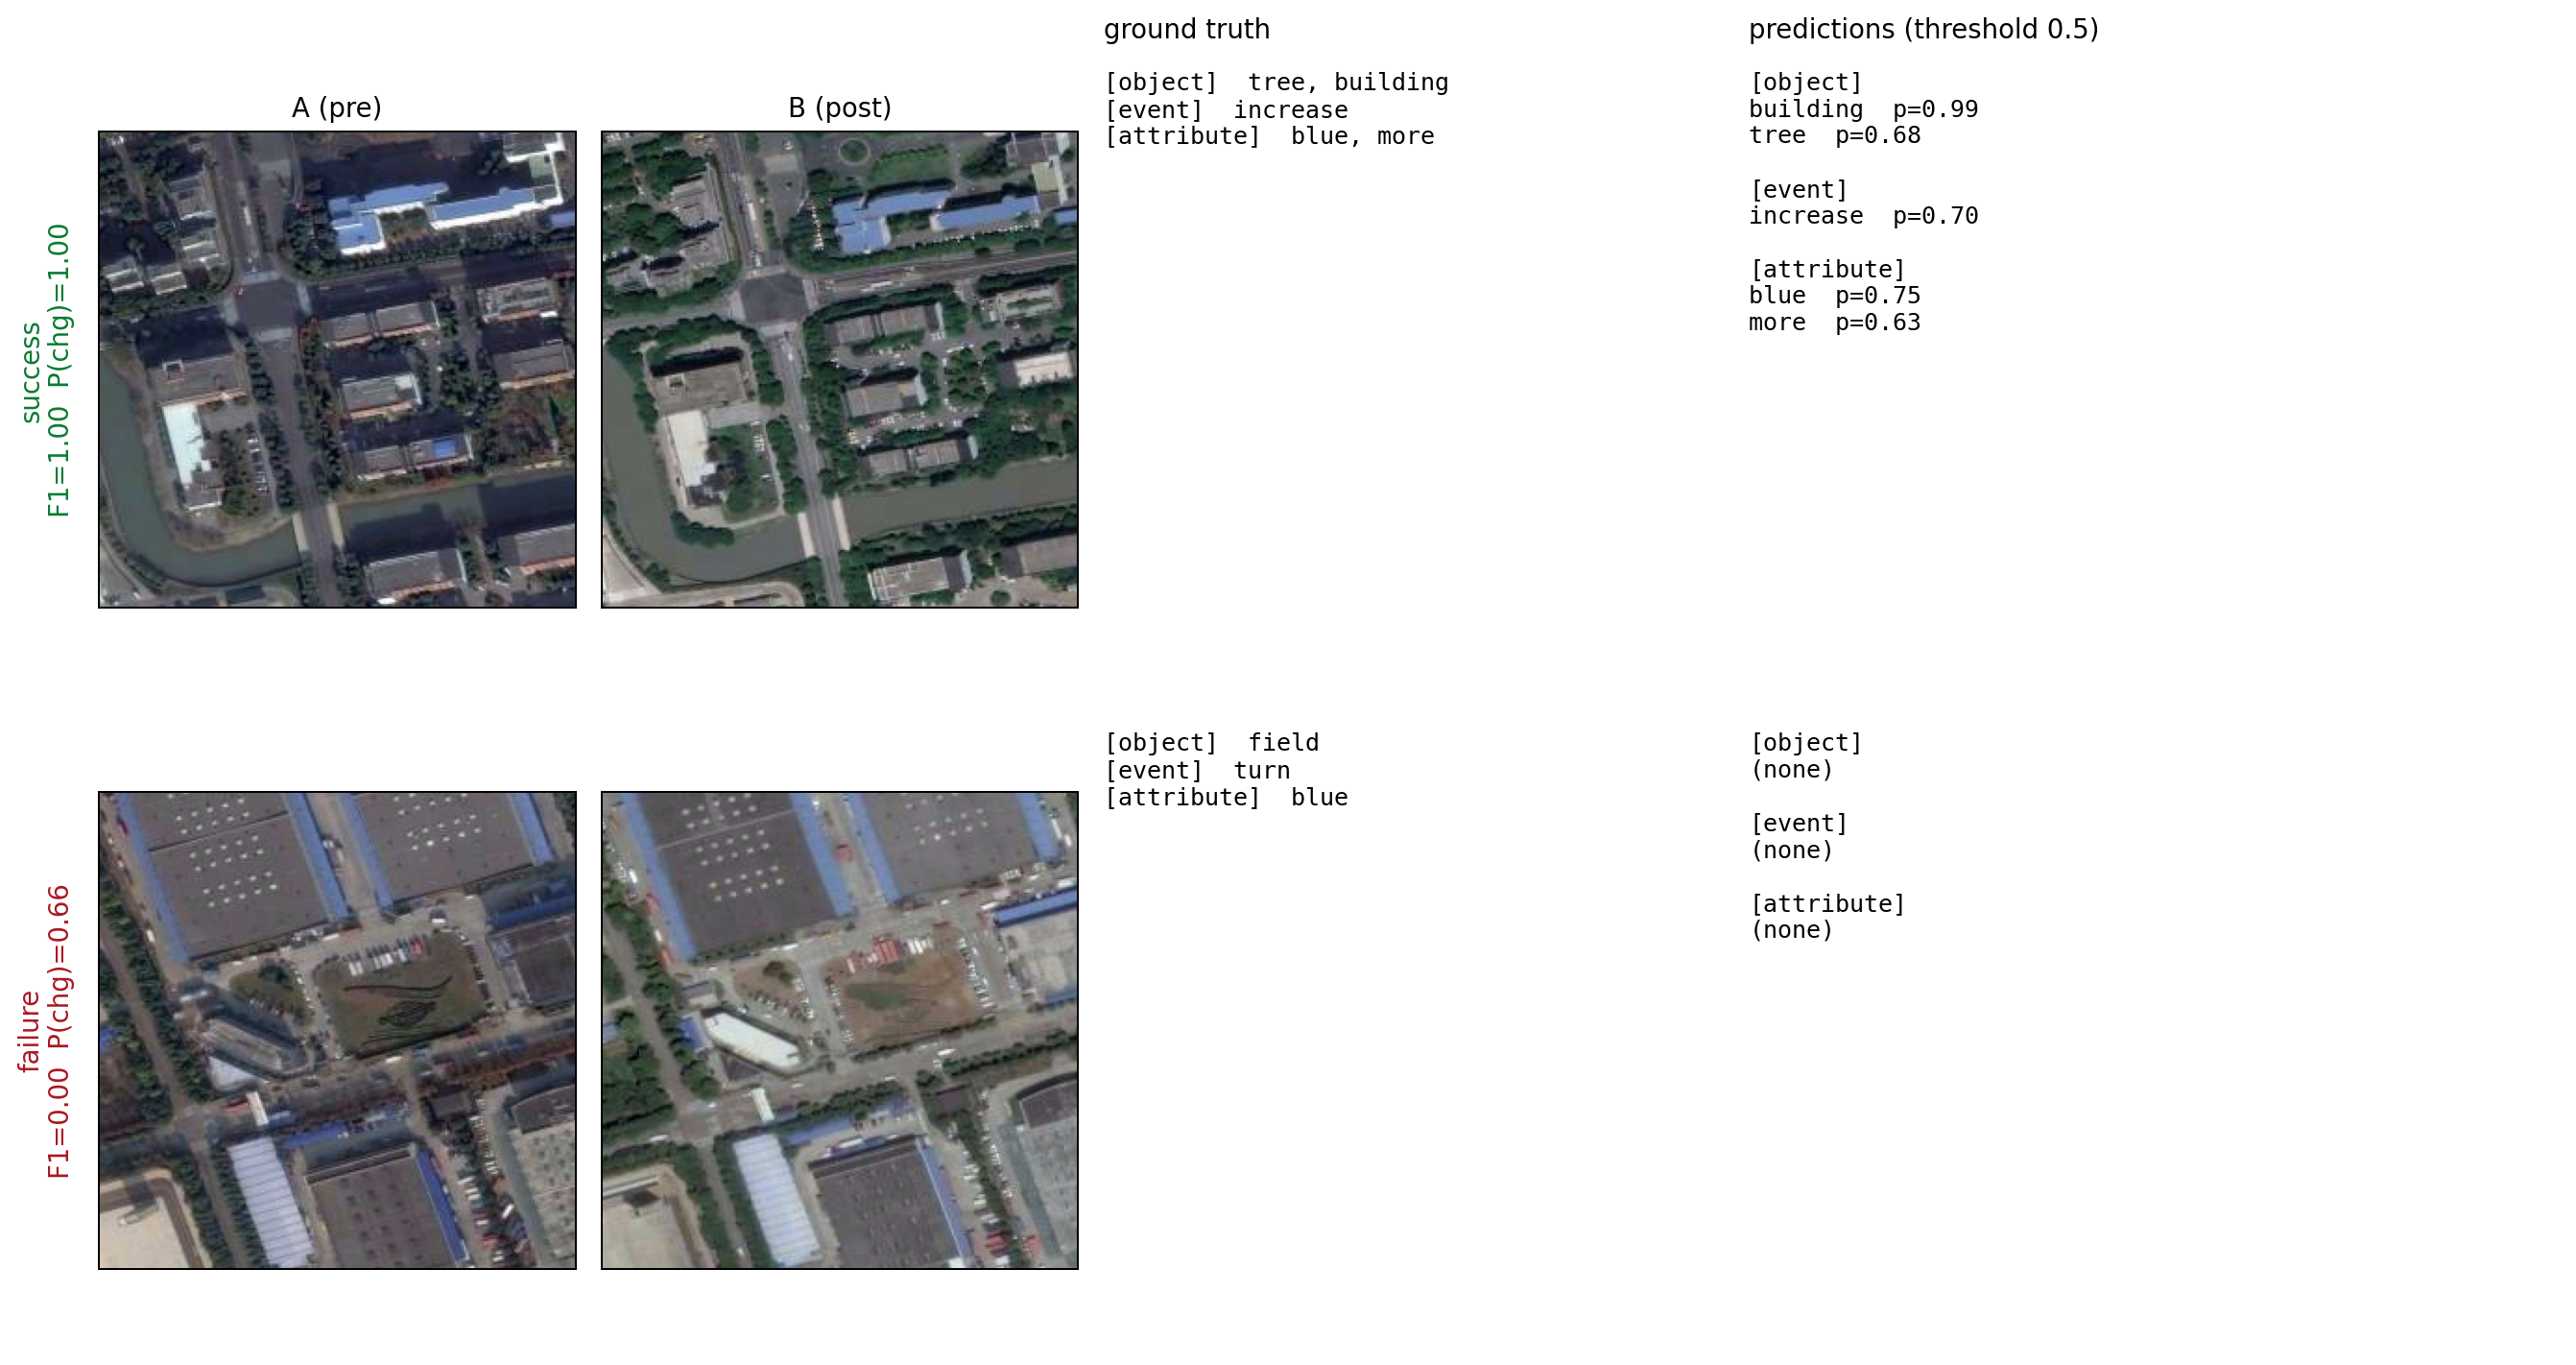
\includegraphics[width=\linewidth]{teaser.png}
  \caption{Bitemporal change classification: given $(A, B)$ the model
    predicts 48 sigmoid labels across three families. Successful and
    failed test pairs are shown side-by-side with predicted probabilities.}
  \label{fig:teaser}
\end{figure}

% Why bitemporal multi-label change is harder than standard change
% detection. The 3-family decomposition. Class imbalance. Our contributions:
% (1) ConvNeXt-V2 backbone choice motivated by a controlled ResNet-50
% baseline, (2) BIT fusion + uncertainty about whether Q2L/UWL helps,
% (3) honest negative results.

% =====================================================================
\section{Related Work}
% 0.4 page.

% Change detection: BIT \cite{chen2022bit} and contemporaries.
% Multi-label classification: ASL \cite{ridnik2021asl}, Q2L \cite{liu2021q2l}.
% Long-tail: DBLoss \cite{wu2020dbloss}.
% Multi-task weighting: Kendall et al. \cite{kendall2018uwl}.
% Modern backbone: ConvNeXt-V2 \cite{woo2023convnextv2}.

% =====================================================================
\section{Method}
% 1.3 pages.

\subsection{Shared Architecture}
% Siamese encoder around ConvNeXt-V2 Tiny pre-trained with FCMAE
% \cite{woo2023convnextv2} at 224x224. Both views concatenated along the
% batch axis and forwarded in a single pass; outputs split back into
% $(f_A, f_B) \in \mathbb{R}^{B \times 768 \times 7 \times 7}$.

\subsection{Phase 1: single-task heads}
% Per family: GAP -> 4-way fusion
% $[f_A; f_B; |f_A - f_B|; f_A \odot f_B] \in \mathbb{R}^{4 \times 768}$
% -> LayerNorm-MLP at width 512 -> linear classifier with sigmoid outputs.
% Auxiliary 1-d head predicts P(change). Loss: Asymmetric Loss
% \cite{ridnik2021asl} with gamma_neg=4, gamma_pos=0, clip=0.05, plus
% BCE on the auxiliary head at weight 0.2.

\subsection{Phase 2: unified multi-task model}
% Same encoder. The GAP+4-way fusion is augmented (not replaced) by BIT:
% L=4 learnable tokens per phase, joint pre-LN transformer (2 layers,
% nhead=8), then cross-attention back to each phase's spatial map. The
% refined spatial maps go through the same 4-way GAP+MLP head. Family
% heads share memory $[\,\text{feat}\,|\,\text{refined\_tokens}\,]$.
% Three configurable axes: fusion in {bit, passthrough}, heads in
% {linear, query2label}, multi-task aggregation in {fixed, uncertainty}.
% Default Phase~2 uses BIT + linear heads + fixed weights
% $\{1, 1, 1, 0.2\}$, matching the Phase~1 aggregation pattern.

\subsection{Training recipe}
% AdamW \cite{loshchilov2019adamw}, head LR 3e-4, backbone LR 3e-5
% (Phase 1) or 2e-5 (Phase 2), LLRD 0.8, weight decay 0.05, cosine
% schedule with 3- or 4-epoch warmup. Mixed precision (bf16) on RTX 5070.
% EMA decay 0.999 with 1000-step warmup. Gradient clip 1.0. Sampling:
% weighted random with $w_i = 1/\sqrt{1 + n_\text{pos}(i)}$ over the
% target family (Phase 1) or the union of all three (Phase 2).
% Augmentation: pair-aware spatial flip/rotate/affine + photometric
% jitter + CutMix at probability 0.3. Three seeds: 42, 1337, 2024.

\begin{figure*}[t]
  \centering
  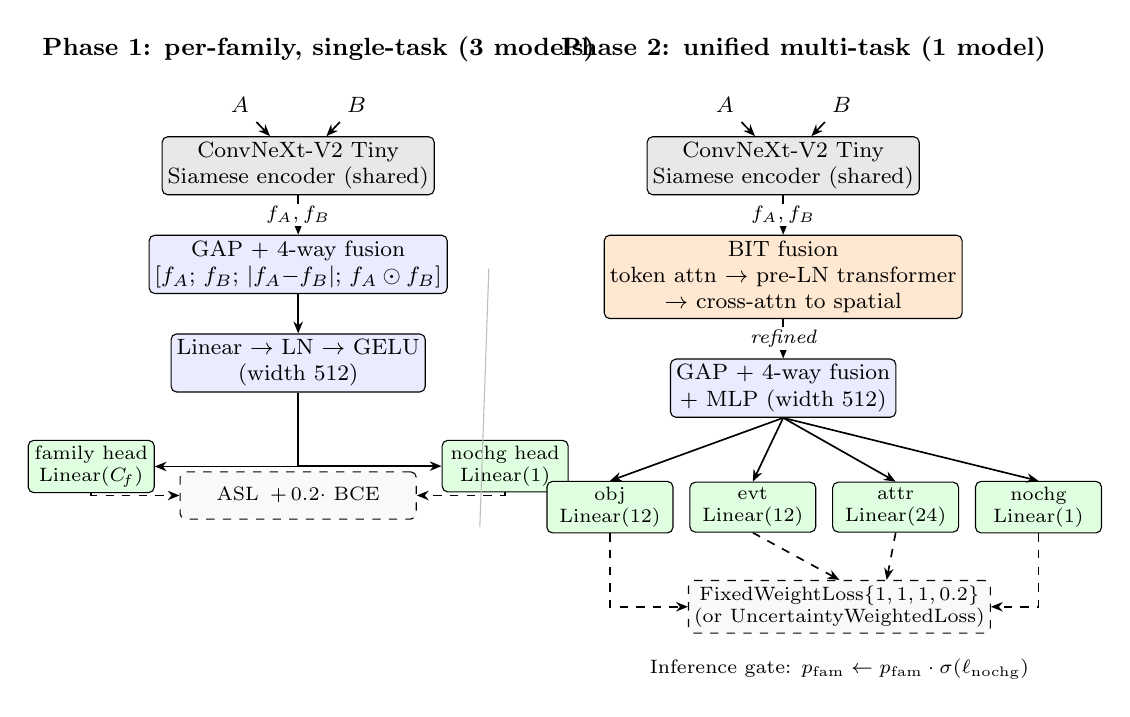
\begin{tikzpicture}[node distance=5mm and 6mm]

    % ---------- Phase 1 (left column) ----------
    \node[io] (p1A) {$A$};
    \node[io, right=10mm of p1A] (p1B) {$B$};
    \node[enc, below=4mm of $(p1A)!0.5!(p1B)$] (p1enc)
      {ConvNeXt-V2 Tiny\\Siamese encoder (shared)};
    \node[fuse, below=of p1enc] (p1fuse)
      {GAP $+$ 4-way fusion\\$[f_A;\,f_B;\,|f_A{-}f_B|;\,f_A\odot f_B]$};
    \node[fuse, below=of p1fuse] (p1mlp)
      {Linear $\to$ LN $\to$ GELU\\(width 512)};
    \node[head, below left =6mm and 2mm of p1mlp] (p1head)
      {family head\\Linear($C_{\!f}$)};
    \node[head, below right=6mm and 2mm of p1mlp] (p1nc)
      {nochg head\\Linear(1)};
    \node[loss, below=10mm of p1mlp] (p1loss)
      {ASL $\,+\,0.2\cdot$ BCE};

    \draw[arr] (p1A) -- (p1enc);
    \draw[arr] (p1B) -- (p1enc);
    \draw[arr] (p1enc) -- (p1fuse) node[label] {$f_A,f_B$};
    \draw[arr] (p1fuse) -- (p1mlp);
    \draw[arr] (p1mlp.south) |- (p1head.east);
    \draw[arr] (p1mlp.south) |- (p1nc.west);
    \draw[arr, dashed] (p1head.south) |- (p1loss.west);
    \draw[arr, dashed] (p1nc.south)   |- (p1loss.east);

    \node[font=\bfseries\small, above=2mm of p1A,
      xshift=10mm, anchor=south]
      {Phase~1: per-family, single-task (3 models)};

    % ---------- Phase 2 (right column) ----------
    \node[io, right=42mm of p1B] (p2A) {$A$};
    \node[io, right=10mm of p2A] (p2B) {$B$};
    \node[enc, below=4mm of $(p2A)!0.5!(p2B)$] (p2enc)
      {ConvNeXt-V2 Tiny\\Siamese encoder (shared)};
    \node[bit, below=of p2enc] (p2bit)
      {BIT fusion\\token attn $\to$ pre-LN transformer\\
        $\to$ cross-attn to spatial};
    \node[fuse, below=of p2bit] (p2mlp)
      {GAP $+$ 4-way fusion\\$+$ MLP (width 512)};
    \node[head, below=8mm of p2mlp, xshift=-22mm] (p2obj)  {obj\\Linear(12)};
    \node[head, right=2mm of p2obj]                (p2evt) {evt\\Linear(12)};
    \node[head, right=2mm of p2evt]                (p2attr){attr\\Linear(24)};
    \node[head, right=2mm of p2attr]               (p2nc)  {nochg\\Linear(1)};
    \node[loss, below=6mm of p2evt, xshift=11mm]   (p2loss)
      {FixedWeightLoss$\{1,1,1,0.2\}$\\(or UncertaintyWeightedLoss)};

    \draw[arr] (p2A) -- (p2enc);
    \draw[arr] (p2B) -- (p2enc);
    \draw[arr] (p2enc) -- (p2bit) node[label] {$f_A,f_B$};
    \draw[arr] (p2bit) -- (p2mlp) node[label] {refined};
    \draw[arr] (p2mlp.south) -- (p2obj.north);
    \draw[arr] (p2mlp.south) -- (p2evt.north);
    \draw[arr] (p2mlp.south) -- (p2attr.north);
    \draw[arr] (p2mlp.south) -- (p2nc.north);
    \draw[arr, dashed] (p2obj.south)  |- (p2loss.west);
    \draw[arr, dashed] (p2evt.south)  -- (p2loss.north);
    \draw[arr, dashed] (p2attr.south) -- ($(p2loss.north)+(6mm,0)$);
    \draw[arr, dashed] (p2nc.south)   |- (p2loss.east);

    \node[font=\bfseries\small, above=2mm of p2A,
      xshift=10mm, anchor=south]
      {Phase~2: unified multi-task (1 model)};

    % Inference gate annotation
    \node[font=\scriptsize, below=2mm of p2loss, align=center]
      {Inference gate: $p_{\text{fam}} \leftarrow p_{\text{fam}} \cdot
        \sigma(\ell_{\text{nochg}})$};

    % Vertical separator between the two phases
    \draw[gray!50, thin] ($(p1mlp.east)+(8mm,12mm)$) --
      ($(p1loss.east)+(8mm,-4mm)$);

  \end{tikzpicture}
  \caption{Phase~1 (left) and Phase~2 (right). Both share the ConvNeXt-V2
    Tiny Siamese encoder. Phase~1 trains three independent models, one
    per label family, with a four-way fusion vector feeding a small MLP
    and a sigmoid family head. Phase~2 keeps the same encoder, inserts
    a Bitemporal Image Transformer (BIT) fusion before the same MLP,
    and emits four heads (three family logits and one no-change scalar)
    aggregated with fixed task weights. The Query2Label heads and
    uncertainty-weighted loss explored as a full-stack ablation are
    drop-in replacements for the linear heads and FixedWeightLoss.}
  \label{fig:arch}
\end{figure*}

% =====================================================================
\section{Experiments}
% 0.4 page.

\subsection{Dataset and splits}
% Bitemporal aerial RGB pairs, frozen train/val/test split. 28% of pairs
% are no-change (all-zero labels in every family). Per-family class
% imbalance is summarized in Table~\ref{tab:eda} (TODO: include EDA
% summary numbers). A leakage check confirms no base filename spans
% multiple splits.

\subsection{Evaluation}
% Macro-F1 (primary), micro-F1, precision/recall (macro), mAP.
% Default decision threshold 0.5 is used unless a row explicitly tunes
% per-class thresholds on the validation split. Test-time augmentation
% (TTA) averages probabilities over {orig, hflip, vflip, rot180}.
% Phase~2 inference applies a multiplicative no-change gate:
% $p^\text{gated}_\text{fam} = p_\text{fam} \cdot p_\text{chg}$.

% =====================================================================
\section{Results}
% 1.8 pages.

\subsection{Main results}
% Table I: Phase 1 and Phase 2 canonical results, 3-seed mean +/- std.

\begin{table}[t]
  \caption{Main results on the test split (EMA weights, default 0.5,
    TTA). 3-seed mean $\pm$ std. Best Phase column per row in bold.}
  \label{tab:main}
  \centering
  \begin{tabular}{lcccc}
    \toprule
    Family & Phase~1 & Phase~2 & $\Delta$ & \\
    \midrule
    Object & TODO & TODO & TODO & \\
    Event & TODO & TODO & TODO & \\
    Attribute & TODO & TODO & TODO & \\
    \midrule
    Mean & 0.277 & 0.282 & +0.005 & \\
    \bottomrule
  \end{tabular}
\end{table}

\subsection{Ablations}
% Table II: 9-row ablation. Walk through:
% (1) A1 -> P1 canonical: ConvNeXt-V2 vs ResNet-50.
% (2) +TTA: small but consistent.
% (3) +gate: null result -- multiplicative gate from the auxiliary head
%     does not help (-0.003).
% (4) DBLoss: 0.5 is uncalibrated (0.266 vs 0.303), per-class threshold
%     tuning recovers most of the gap (0.285) but does not overtake ASL.
% (5) P1 -> P2 canonical: BIT fusion contributes +0.005 mean and
%     halves the cross-seed std (0.029 -> 0.013).
% (6) P2 full stack (Q2L + UWL): underperforms both no-BIT and
%     canonical Phase~2 even after 50 epochs (early-stop cap).

\begin{table*}[t]
  \caption{Ablation. 3-seed mean $\pm$ std macro-F1. DBLoss row is
    object-only (the heaviest 270:1 imbalance family).}
  \label{tab:ablation}
  \centering
  % TODO: paste rows from results/ablation_table.md
  \begin{tabular}{lcccc}
    \toprule
    Variant & Object & Event & Attribute & Mean \\
    \midrule
    A1: ResNet-50 + ASL & TODO & TODO & TODO & TODO \\
    P1: ConvNeXt-V2 + ASL (canonical) & 0.303 & 0.272 & 0.258 & \textbf{0.277} \\
    \vdots & & & & \\
    \bottomrule
  \end{tabular}
\end{table*}

\subsection{Per-class behaviour and qualitative examples}

\begin{figure}[t]
  \centering
  \includegraphics[width=\linewidth]{phase2_object_per_class_f1.png}
  \caption{Per-class F1 on the test split for the Phase~2 object family,
    sorted by descending mean across 3 seeds. Bars show mean $\pm$ std.
    Rare classes -- visible at the bottom of the chart -- score
    consistently lower; the long tail dominates the macro-F1 loss.}
  \label{fig:perclass}
\end{figure}

\begin{figure}[t]
  \centering
  \includegraphics[width=\linewidth]{phase2_curves.png}
  \caption{Phase~2 canonical training dynamics across 3 seeds: train
    loss, val loss, per-family val macro-F1 (curves) and their mean
    (heavy line). Shaded bands are $\pm 1$ std.}
  \label{fig:curves}
\end{figure}

\begin{figure}[t]
  \centering
  \includegraphics[width=\linewidth]{phase2_qualitative.png}
  \caption{Qualitative test examples from the canonical Phase~2 model
    (seed 42). Top rows: two best-F1 samples; bottom rows: two failure
    cases with at least one positive ground-truth label. Each row shows
    $(A, B, \text{ground truth}, \text{predictions with probabilities})$.}
  \label{fig:qual}
\end{figure}

% =====================================================================
\section{Conclusion}
% 0.2 page. 1 paragraph. Restate the key finding (BIT fusion's modest
% mean gain + variance reduction is the headline; the long-tail object
% family remains the bottleneck; honest negative results on Q2L/UWL/gate
% inform what NOT to add at this dataset scale).

% =====================================================================
\bibliographystyle{IEEEtran}
\bibliography{refs}

\end{document}
